Pour plannifier ce projet, nous avons travaillé sur le site teamwork.com qui nous permets de gérer un planning, mais aussi
les tâches assignées à chacun pour la journée et leurs avancement. Nous avons tout d'abord créer un planning "global" qui
représente le travail à effectuer du début du projet jusqu'à la fin du projet. Ce planning a bien entendu été 
validé par nos clients et notre reponsable industriel. Nous avons rencontré beaucoup de difficultés pour créer
ce planning : \\
\begin{itemize}
\item Nous ne savions pas trop au début comment nous allions nous organiser. \\
\item Nous ne savions pas du tout comment nous allions procéder, si nous allions utiliser par exemple une méthode agile comme décrit en cours \\
\end{itemize}

Au final nous avons abouti à un planning général qui à la forme suivante :\\
\begin{itemize}
\item \texttt{Du 19/01 au 07/02:} écrire toutes les spécifications, le workflow, les règles de programmation, mettre en place l'équipe. Notre
but durant cette période était de bien mettre en place le projet, bien discuter avec les clients pour cerner les différents 
problèmes spécifiés précédemment (langage de programmation par exemple). Cette période peut paraître longue mais elle
ne contient que trois semaines dont une semaine de départ au ski pour certains. \\
\item \texttt{Du 07/02 au 07/03 :} développement en suivant une méthode agile comme vu en cours, plus précisemment une méthode
"scrum". Ce point sera développé dans la suite. Nous avons, dans cette période de un mois, posé deux dates importantes
"milestones" auquelles nous devons présenté une version stable du projet : le 20/02 et le 27/02.\\
\item \texttt{Du 07/03 au 13/03 :} (soutenance) : préparer la soutenance.\\
\end{itemize}



	Ce planning trés général est bien sur beaucoup plus détaillé sur le site sur lequel nous avons, pour chaque journée, défini les tâches
à effectuer (beaucoup trop pour l'inclure dans ce rapport). La rédaction et la mise en place de ce planning, bien que trés général nous a pourtant posé de nombreux problèmes. Nous 
ne pensions par exemple pas passer autant de temps sur la rédaction des spécifications. En fait, le simple fait de ne pas avoir fait de 
planning au début nous a fait perdre beaucoup de temps, c'est ainsi que l'on s'est rendu compte de l'importance 
d'un planning dans la gestion de projet. En effet, le fait de ne pas avoir de date butoire aprés laquelle nous imposions au client
de ne plus modifier les spécifications a fait que nous modifions sans cesse les spécifications. Alors que nous aurions du dire au client que 
dépassé une certaine date, il ne serait plus possible de modifier les spécifications. 


	Nous allons maintenant détaillé la période de développement. Aprés les premières discussions avec l'un de nos client, nous nous 
sommes rendu compte que celui ci n'étais pas trés clair dans ces attentes, et surtout qu'il n'avais pas l'air trés sur d'une part de 
ce que nous étions capables de developper en un mois et d'autre part de ce qu'il voulait vraiment que l'on fasse. Ainsi, il nous a paru 
évident qu'il faudrait utiliser uné méthode agile pour itérer sur les attentes du client au fur et à mesure de l'avancement
du projet. Nous avons, plus précisemment, utiliser une méthode "scrum", qui impose donc que nous avions des réunions toutes les semaines 
avec les clients. Lors de chaque réunion, nous devons présenté ce que l'on avait fait lors de la semaine, ce que nous ferons les semaines prochaines, 
et enfin les problèmes que nous avons. Ainsi nous avons créer un planning un peu plus détaillé pour chacune de ces semaines de développement :

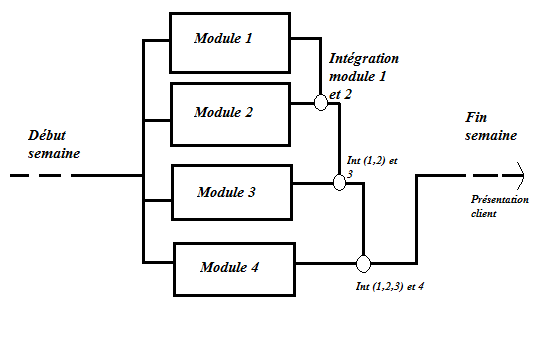
\includegraphics[scale=1]{planning.png}


Nous avons en fait découper le travail à effectuer par chacun en module. Chacun, du lundi au mercredi, développe son module, puis le jeudi, on intègre
ces modules l'un aprés l'autre, puis l'on présente ceci le vendredi. Chaque vendredi on a donc une nouvelle version intermédiaire du projet. Comme 
expliqué précedemment, nous avons deux dates importantes qui représentent des versions stables.